\documentclass[12pt]{article}
\usepackage{graphicx}
\usepackage[colorlinks=true, pdfborder={0 0 0}, linkcolor=blue, urlcolor=blue, citecolor=blue]{hyperref}
\usepackage[a4paper, margin=.8in]{geometry}
\usepackage{float}
\usepackage{amsmath}
\usepackage{amssymb}
\usepackage{anysize}
\usepackage{caption}
\usepackage{tcolorbox}
\usepackage{titlesec}
\usepackage{ulem}

\titleformat{\section}{\normalfont\LARGE\bfseries}{\thesection}{1em}{}
\titleformat{\subsection}{\normalfont\Large\bfseries}{\thesubsection}{1em}{}
\titleformat{\subsubsection}{\normalfont\large\bfseries}{\thesubsubsection}{1em}{}

\titlespacing*{\subsubsection}{0pt}{.8em}{.3em}

\renewcommand{\ULthickness}{1pt}
\renewcommand{\ULdepth}{0.5ex}  

\begin{document}
  

\fontsize{14}{16}
\selectfont
\captionsetup[figure]{font=normal}
\newtcolorbox{note}[1][]{colback=white, colframe=black, sharp corners, boxrule=0.3mm, #1}
\newtcolorbox{block}[1][left=1cm, top=-.2cm, bottom=-.2cm]{colback=white, colframe=white, sharp corners, boxrule=0.3mm, #1}

\title{Lasers}
\author{Sudarsan D Naidu}
\maketitle

\tableofcontents

\section{Introduction}

In this chapter, we will explore how lasers work. However, before understanding the mechanism of lasers, we need to learn about the concept of energy levels, the interaction between radiation and matter, population distribution, Einstein coefficients, and more.

\subsection{Energy Level}

An energy level is a specific, quantized state that an $e^{-}$ can occupy in an atom or molecule, each with a fixed energy value. We will be studying about these energy levels in depth when we will be learning Quantum Physics. \vspace{.2cm}

\uline{What does an atom getting excited mean?} An atom getting excited means that the atom has gained some energy (relative to its ground state). When an electron of the atom get excited, it gains energy and as an electron is part of an atom, so the atom too does gain energy. From whatever we know till now, when a photon is absorbed by an atom, it is more accurate to say that the electron has been excited. But, in this chapter, we will often keep atom as our point of reference. So, whenever we say that an atom has been excited, we refer to excitation of the outermost valence shell electron. Refer to Born-Oppenheimer approximation for a better idea on how nucleus of an atom is not affected when the photon is absorbed by the atom.

\begin{quote}
    If an electron has been excited, then the atom too gets excited but if an atom has been excited, there are many possibilities. But, in this chapter, we will be only considering the excitation of the outermost valence shell electron as the only possibility.
\end{quote}

\subsection{Energy Gap}

Usually for an \textbf{isolated gaseous atom}, there are many energy levels in discrete which the electron can occupy. But, in the case of solids, due to tightly packed atoms and their orbital overlap, the discrete energy levels become very close and appear to be continuous. Such continuous energy levels are called as energy bands and the $e^{-}$ can take any energy value between the lowest and highest value of energy band. The concept of energy bands will be discussed again in Band Theory of Solids in depth.

\subsection{Classical Representation of Atom}

In classical view (an extended version of Newtonian mechanics), these energy levels are related with the orbits of the $e^{-}$ revolving around the nucleus (See figure 1).

\begin{figure}[H]
    \centering
    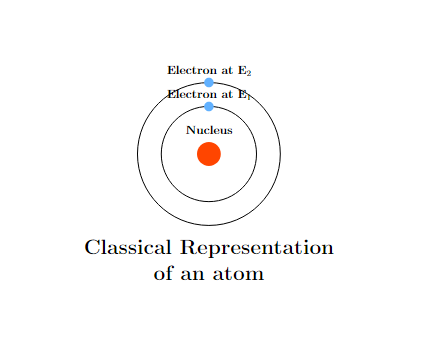
\includegraphics[scale=0.8]{./img/01_classical_atom.png}
    \caption{Classical Representation of an Atom}
\end{figure}

This idea is very outdated and is wrong as we move towards the concept of Quantum Mechanics. The atom is often represented like this in some books to keep things simple. In the quantum mechanical model of the atom, we consider electrons to be in the orbitals corresponding to their energy levels.

\subsection{Energy Level Diagrams}

To explain phenomena related to interaction between radiation and matter, we need a good diagrammatic representation of an atom. As stated earlier, we are not interested in outdated classical representation of atom anymore in favour of the quantum mechanical model. \vspace{.2cm}

Now, if we follow the quantum mechanical model, representing orbitals in an atom is highly complicated, making it even more challenging to use those diagrams to explain certain phenomena. We have discussed earlier that in this chapter we are going to equate energy states of an atom with the energy state of its outermost valence electron, i.e. when an electron excites from $E_{1}$ to $E_{2}$, the atom too excites from $E_{1}$ to $E_{2}$. So, instead of using diagrams of electrons, orbitals or orbits, we will be using the diagram of energy levels (see figure 2) to explain several phenomena.

\begin{figure}[H]
    \centering
    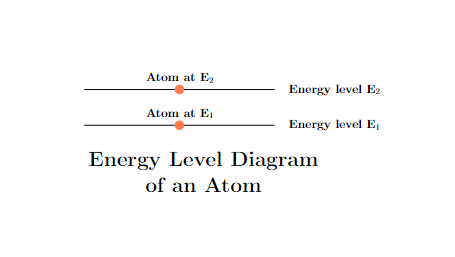
\includegraphics[scale=0.8]{./img/02_energy_levels.png}
    \caption{Energy level diagram of an Atom}
\end{figure}

This energy level diagram helps use to visualise in which energy state the atom (or its outermost valence shell $e^{-}$) is in without violating any idea of quantum mechanical model of an atom. Compare figure 2 with figure 1.

\subsection{References}

\begin{itemize}
    \item Read Basavaraju's book on Engineering Physics for fundamental ideas (Chapter 5 Lasers)
    \item Watch this \href{https://www.youtube.com/watch?v=_JOchLyNO_w&t=233s}{YT video} for a complete animated video of the whole mechanism of LASER. The only con of this video will be its attempt of using the classical representation of atom in it.
    \item See this \href{https://www.reddit.com/r/Physics/comments/1ev7gss/are_energy_levels_for_electrons_or_atoms/}{Reddit post} for question on energy levels.
\end{itemize}

This page has to be updated once we complete studying Quantum Physics and its mechanics.

\section{Types of Interactions}

Working of laser depends on the three different ways of interaction of radiation and matter. In this chapter, there will only be an introduction to the interactions and will study them later in depth in Quantum Mechanics. \textbf{Note} that these interactions happen only in isolated atoms with discrete $E$ levels.

\subsection{Stimulated Absorption}

This interaction is also called as \textbf{Induced Absorption} in some books (like in Basavaraju's) while in some others, it is called as \textbf{Stimulated Absorption}.

\begin{figure}[H]
    \centering
    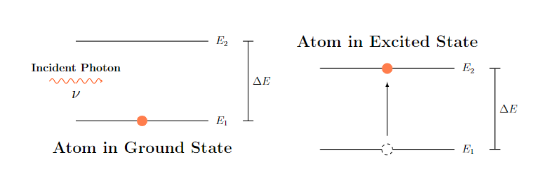
\includegraphics[scale=0.8]{./img/03_induced_absorption.png}
    \caption{Stimulated Absorption}
\end{figure}

Here (and for the other 2 interactions too), assume $E_{1}$ is the ground state and $E_{2}$ is some excited state of that atom.

\begin{equation}
    \Delta E = E_{2} - E_{1}
\end{equation}

\textbf{Note} although $E_{1}$ will be greater than $E_{2}$ in magnitude but their values are in negative thus making the $\Delta E$ positive. \vspace{.2cm}

Here, the photon is absorbed by the atom to excite itself from the ground state to an excited state. This is only possible if the energy of photon is same as the energy different between two levels. So, by \textbf{Planck's formula}.
\begin{equation}
    \Delta E = h\nu
\end{equation}

\subsection{Spontaneous Emission}

\begin{figure}[H]
    \centering
    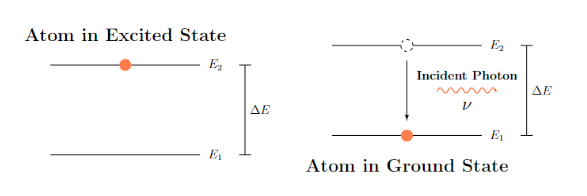
\includegraphics[scale=0.8]{./img/04_spontaneous_emission.png}
    \caption{Spontaneous Emission}
\end{figure}

Any atom in an excited state is unstable and tends to de-excite to the ground state without any external aid (thus spontaneous). During this process, it emits an photon of an energy equal to the energy difference. \textbf{Note} that, there is an universal tendency for any system to be in the lowest energy state to keep itself stable.

Photons emitted by two atoms excited under (and are in) identical conditions undergoing spontaneous emission, \textbf{will not have any phase relationship} (i.e. in any direction and can have phase differences). So, photons emitted under this process are incoherent (i.e. no phase relationship). Such incoherent emissions can be seen in Thermoionic emission in bulb, candle flame, etc.

\subsection{Stimulated Emission}

\begin{figure}[H]
    \centering
    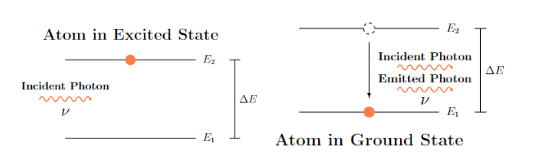
\includegraphics[scale=0.8]{./img/05_stimulated_emission.png}
    \caption{Stimulated Emission}
\end{figure}

Although, atoms can get de-excited without any external aid as seen in Spontaneous emission, they can also get de-excited by an incident photon of an energy equal to the energy difference between the excited levels. When such de-excitation happens, the atom emits another photon which will be in phase (i.e. coherent) with the incident photon. This process is also referred to as "negative absorption".

\section{Population distribution of Atoms in Excited states}

In a system, let $n_{i}$ be the number density (i.e. number of units per unit volume) of atoms existing in the energy state $i$. To keep things more simple in understanding the lasing process, we will use the energy level diagrams to show the distribution of atoms of system in the excited states (see figure 6). Also, by "population", we mean the "number" of atoms.

\begin{figure}[H]
    \centering
    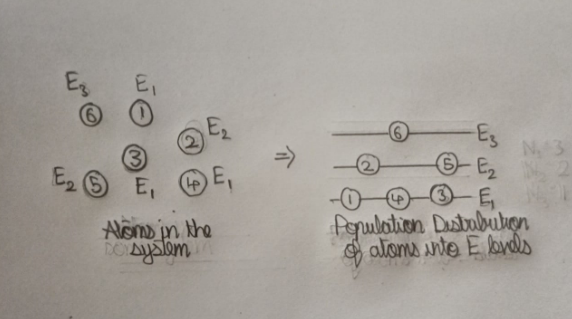
\includegraphics[scale=.8]{./img/06_population_dist.png}
    \caption{Population distribution of atoms in the system}
\end{figure}

\textbf{Note} that population distribution is only for identical atoms. In real systems, the number of atoms exceed the number of energy levels possible in that system. (??)

\subsection{Rate of change of Population Density}

Then, $dn_{i}/dt$ will be the rate at which the number density of atoms exciting or de-exciting (depending on the sign of the derivative) from/to an energy state $i$. \vspace{.2cm}

Let's consider a system having energy states $E_{1}$, $E_{2}$, ..., $E_{i}$. Let it have a total population density (of atoms) $n$,
\begin{equation}
    n_{1} + n_{2} + ... + n_{i} = n
\end{equation}

We can differentiate this equation (w.r.t $t$) to get a relation between the rate of atoms exciting and de-exciting in each energy state,

\begin{equation*}
    \frac{dn_{1}}{dt} + \frac{dn_{2}}{dt} + ... + \frac{dn_{i}}{dt} = \frac{dn}{dt}
\end{equation*}

In a fixed system, we can assume $n$ to be constant, which makes $dn/dt$ to be 0,
\begin{equation*}
    \frac{dn_{1}}{dt} + \frac{dn_{2}}{dt} + ... + \frac{dn_{i}}{dt} = 0
\end{equation*} 

In transition of atoms, involving only two states, the rates of other states will become zero,
\begin{align}
    \frac{dn_{1}}{dt} + \frac{dn_{2}}{dt} & = 0 \notag \\
    \Rightarrow \frac{dn_{2}}{dt} & = -\frac{dn_{1}}{dt}
\end{align}

\subsection{Thermodynamic Equilibrium}

At Thermodynamic Equilibrium, the net energy exchanged will be 0 (energy exchange will happen but the sum will be 0). Excitation and de-excitation of atoms are energy exchanges too as they involve absorbing and emitting radiation (energy), so at Thermodynamic Equilibrium, the net change in the number of excited atoms will be 0 too. \vspace{.2cm}

This means, for any state $i$ at Thermodynamic Equilibrium, 

\begin{equation}
    \frac{dn_{i}}{dt} = 0
\end{equation}

\subsection{Boltzmann Factor}

At Thermodynamic Equilibrium, energy states having large population densities can be related with each other by the Boltzmann factor,

\begin{equation}
    \frac{n_{2}}{n_{1}} = e^{-\frac{E_{2} - E_{1}}{kT}}
\end{equation}

This formula is built on approximation of the theoretical data and works only for large $n$ values. \vspace{.2cm}

The derivation of this equation is given \href{https://www.phys.ufl.edu/~meisel/Boltzmann.pdf}{in this paper}.

\subsection{Non Thermodynamic Equilibrium Conditions}

We know in energy level scheme, $E_{2} > E_{1}$. By substituting this inequality in Boltzmann's equation in (6), we get $n_{2} < n_{1}$. If we place the system at a very huge temperature (i.e. $T \rightarrow \infty$ but in equilibrium), then from equation (6), we get $n_{2} \rightarrow n_{1}$. \vspace{.2cm}

As Boltzmann's equation is only valid at Thermodynamic Equilibrium, we can say $n_{2}$ is always lesser than or equal to $n_{1}$ (i.e $n_{2} \le n_{1}$) under Thermodynamic Equilibrium. In short, $n_{2}$ can never be greater than $n_{1}$ under Thermodynamic Equilibrium conditions. 
\begin{equation*}
    n_{2} \le n_{1} \text{ (under Thermodynamic Equilibrium)}
\end{equation*}

So, to make $n_{2} > n_{1}$, we have to feed energy in other ways to the system resulting in non equilibrium conditions which is essential for Lasing process (will be discussed later). 

\section{Einstein's Coefficients}

The formation of atomic spectral lines is due to the three different interactions of radiation and matter which was proposed by Einstein in 1916. In his studies, he assumed matter is in Thermodynamic Equilibrium (see 3.2) with Black Body radiation. \vspace{.2cm}

Each of these processes (interactions) proposed by Einstein are associated with an Einstein coefficient. Einstein considered the case of isotropic radiation of frequency $\nu$ (i.e. having same frequency in all directions the radiation is propagating at) and spectral energy density $\rho(\nu)$. \vspace{.2cm}

Read more about this \href{https://en.wikipedia.org/wiki/Einstein_coefficients}{in Wikipedia}.

\subsection{Spectral Energy Density}

Let radiation of continous spectrum of frequencies be incident on the system. Let $\rho(\nu)d\nu$ be the energy incident per unit volume (i.e. energy density) of the radiations having frequencies between $\nu$ and $\nu + d\nu$ in the spectrum. Here, $\rho(\nu)$ is called as spectral energy density (having dimensions of $E/A\nu$) which is the energy density per frequency of radiations having frequencies between $\nu$ and $\nu + d\nu$. \vspace{.2cm}

Also, in some books (like in Basavaraju's), this has been represented by $U_{\gamma}$ where the frequency is represented by $\gamma$. \textbf{Note} that, this parameter is independent of direction of radiation as we have assumed isotropic frequencies. \vspace{.2cm}

According to \textbf{Planck's law}, the spectral energy density is given as,

\begin{equation}
    \rho(\nu) = \frac{8\pi h\nu^3}{c^3} \frac{1}{e^\frac{h\nu}{kT} - 1}
\end{equation}

We will study about this law later in Quantum Physics.

\subsection{Description of Einstein's coefficients}

Let's consider two energy levels $E_{1}$ (ground state) and $E_{2}$ (some excited state) where $n_{1}$ and $n_{2}$ are the respective population densities of atoms in those energy states. Now, let's see how the three kinds of interactions of radiation and matter are described by the Einstein's coefficients,

\subsubsection{Stimulated Absorption}

In this process, the atoms excite from $E_{1}$ to $E_{2}$ due to the incident radiation of frequency $\nu$. To measure the rate of this process (and for the others too), we will consider $E_{1}$ (ground state) and its population density $n_{1}$ as reference, i.e.,
\begin{align*}
    \text{Rate of stimulated} & = \text{Rate at which atoms are undergoing stimulated} \\
    \text{absorption} & \quad \text{absorption from } E_{1} \text{ to } E_{2} \\ 
    & = (\frac{dn_{1}}{dt})_{st.a.}
\end{align*}

And, from experiments, we know, 
\begin{align*}
    \textnormal{Rate of stimulated absorption} \propto -n_{1}\rho(\nu) \\ 
    (\frac{dn_{1}}{dt})_{st.a.} \propto -n_{1}\rho(\nu)
\end{align*}

As atoms excite from $E_{1}$ to $E_{2}$, it results in decrease in $n_{1}$ (and increase in $n_{2}$) which explains the negative sign. The rate of stimulated absorption will be more if there are more atoms in the ground state $E_{1}$ to get excited to $E_{2}$ so the rate depends on $n_{1}$. This points out the fact that the rate of stimulated absorption will decrease as more and more atoms in $E_{1}$ get excited. Also, as this process is initiated by the energy of the incident radiation, it also depends on the spectral energy density of it. \vspace{.2cm}

The proportional constant for the equation is the Einstein coefficient $B_{12}$ $[m^{3}J^{-1}s^{-2}]$ where $12$ indicates the direction of process (i.e. $E_{1}$ to $E_{2}$) and $B$ indicates the process is stimulated (induced). After plugging the Einstein coefficient in the proportional equation, we get,

\begin{equation}
    (\frac{dn_{1}}{dt})_{st.a.} = -B_{12}n_{1}\rho(\nu) 
\end{equation}

To find the rate at which the atoms are getting excited to $E_{2}$ by stimulated absorption, we can substitute the above rate in the equation (4),

\begin{equation*}
    (\frac{dn_{2}}{dt})_{st.a.} = -(\frac{dn_{1}}{dt})_{st.a.} = B_{12}n_{1}\rho(\nu)
\end{equation*}

\subsubsection{Spontaneous Emission}

In this process, the atoms de-excite from $E_{2}$ to $E_{1}$ spontaneously (i.e. without any external aid). Like we did for stimulated absorption, we are going to consider $E_{1}$ (ground state) as our reference to find rate of this emission.
\begin{align*}
    \text{Rate of spontaneous} & = \text{Rate at which atoms are undergoing spontaneous} \\
    \text{emission} & \quad \text{emission from } E_{2} \text{ to } E_{1} \\ 
    & = (\frac{dn_{1}}{dt})_{sp.e.}
\end{align*}

And, from experiments, we know, 
\begin{align*}
    \textnormal{Rate of spontaneous emission} \propto n_{2} \\ 
    (\frac{dn_{1}}{dt})_{sp.e.} \propto n_{2}
\end{align*}

As atoms de-excite from $E_{2}$ to $E_{1}$, there will be an increase in $n_{1}$ (and decrease in $n_{2}$) which explains why it has no negative sign. The rate of spontaneous emission will be more if there are more excited atoms in $E_{2}$ (i.e. $n_{2}$) to get de-excited spontaneously, so the rate depends on $n_{2}$. As this process is independent of any external aid (i.e. no incident radiation like in stimulated absorption), the rate is independent of spectral energy density. \vspace{.2cm}

The proportional constant for the equation is the Einstein coefficient $A_{21}$ $[s^{-1}]$ where $21$ indicates the direction of process (i.e. $E_{2}$ to $E_{1}$) and $A$ indicates the process is spontaneous. After plugging the Einstein coefficient in the proportional equation, we get,
\begin{equation}
    (\frac{dn_{1}}{dt})_{sp.e.} = A_{21}n_{2}
\end{equation}

We can get the rate of this emission keeping $E_{2}$ as our reference by applying equation (4) like we did earlier in stimulated absorption.

\subsubsection{Stimulated Emission}

In this process, the atoms de-excite from $E_{2}$ to $E_{1}$ due to incident of radiation of frequency $\nu$. Taking $E_{1}$ (ground state) as our reference like we did earlier.
\begin{align*}
    \text{Rate of stimulated} & = \text{Rate at which atoms are undergoing stimulated} \\
    \text{emission} & \quad \text{emission from } E_{2} \text{ to } E_{1} \\ 
    & = (\frac{dn_{1}}{dt})_{st.e.}
\end{align*}

And, from experiments, we know, 
\begin{align*}
    \textnormal{Rate of stimulated emission} \propto n_{2}\rho(\nu) \\ 
    (\frac{dn_{1}}{dt})_{st.e.} \propto n_{2}\rho(\nu)
\end{align*}

Like in spontaneous emission, the atoms get de-excited from $E_{2}$ to $E_{1}$ making the rate dependent on the population density in excited state (i.e. $n_{2}$) and has a positive sign (due to the increase in $n_{1}$). Unlike in spontaneous emission, here the emission takes place because of the incident radiation, so the rate here depends on the spectral energy density of the incident radiation (like in stimulated absorption). \vspace{.2cm}

The proportional constant for the equation is the Einstein coefficient $B_{21}$ $[m^{3}J^{-1}s^{-2}]$ where $21$ indicates the direction of process (i.e. $E_{2}$ to $E_{1}$) and $B$ indicates the process is stimulated. After plugging the Einstein coefficient in the proportional equation, we get,
\begin{equation}
    (\frac{dn_{1}}{dt})_{sp.e.} = B_{21}n_{2}\rho(\nu)
\end{equation}

Again, we can get the rate of this emission keeping $E_{2}$ as our reference by applying equation (4) like we did earlier in stimulated absorption.

\subsection{Probability aspect of Einstein Coefficients}

\subsubsection{Stimulated absorption-only system}

Let's consider a system where atoms only undergo stimulated absorption (no stimulated emission or spontaneous emission) from its $E_{1}$ state to $E_{2}$ state when a radiation of required energy is incident on it. \vspace{.2cm}

In that system, let $P(t)$ be the probability of an atom to undergo stimulated absorption from $E_{1}$ to $E_{2}$ at time $t$ and let $P^c(t)$ be the probability of an atom to remain in the same $E_{1}$ state at time $t$ (i.e. not undergoing any transition), \vspace{.2cm}
\begin{equation}
    P(t) + P^c(t) = 1
\end{equation}

As more and more atoms in $E_{1}$ undergo stimulated absorption to $E_{2}$, the population density $n_{1}$ decreases which means an atom in $E_{1}$ state has more chances (i.e. probability) to absorb the incident radiation and get excited to $E_{2}$. One can imagine it like this: if the supplies are fixed and the number of people in the crowd is decreasing, then it becomes more probable for each person in the crowd to obtain a supply. This explains why is the probability of an atom getting excited or not is a function of time $t$ (i.e. dependent on time $t$). \vspace{.2cm}

We can define the probability of an atom to remain in the same state (i.e. $P^c(t)$) as,
\begin{align}
    \text{Probability of an atom to} & = \text{Ratio of population density of atoms} \notag \\
    \text{remain in the state} & \quad \text{  in that state at t=t to the population} \notag \\
    & \quad \text{  population density at t=0} \notag \\
    \Rightarrow P^c(t) & = \frac{n_{1}(t)}{n_{1}(0)} 
\end{align}

Here, $n_{1}(t)$ is the population density at $E_{1}$ state at time $t$. \vspace{.2cm}

Since we assumed there is only stimulated absorption taking place in the system, the change in population density of atoms in $E_{1}$ is only due to stimulated absorption,

\begin{equation*}
    \frac{dn_{1}}{dt} = (\frac{dn_{1}}{dt})_{st.a.}
\end{equation*} \vspace{.1cm}

Now, we can plug equation (8) into it,
\begin{equation*}
    \frac{dn_{1}}{dt} = -B_{12}n_{1}\rho(\nu) 
\end{equation*}

After rearranging the terms, we can integrate the equation on the LHS from $n_{1}(0)$ to $n_{1}(t)$ and on the RHS from $0$ to $t$, where $n_{1}(t)$ is the population density $n_{1}$ at time $t$,
\begin{align}
    \Rightarrow \frac{dn_{1}}{n_{1}} & = -B_{12}\rho(\nu)dt \notag \\
    \Rightarrow \int_{n_{1}(0)}^{n_{1}(t)} \frac{dn_{1}}{n_{1}} & = \int_{0}^{t} -B_{12}\rho(\nu)dt \notag \\
    \Rightarrow ln(\frac{n_{1}(t)}{n_{0}(0)}) & = -B_{12}\rho(\nu)(t - 0) \notag \\
    \Rightarrow \frac{n_{1}(t)}{n_{1}(0)} & = e^{-B_{12}\rho(\nu)t}
\end{align}

Now, we can substitute the equation (12) into it,
\begin{equation*}
    P^c(t) = e^{-B_{12}\rho(\nu)t}
\end{equation*}

Using equation (11), we can find the value of $P(t)$,
\begin{align}
    P(t) & = 1 - P^c(t) \notag \\
    \Rightarrow P(t) & = 1 - e^{-B_{12}\rho(\nu)t}
\end{align}

Thus, we have arrived at the equation for the probability of an atom undergoing stimulated absorption . \textbf{Note} that this has been derived under the assumption that no other interactions (such as stimulated emission or spontaneous emission) are taking place. In reality (e.g., in the lasing process), all three interactions (i.e. stimulated absorption, stimulated emission, and spontaneous emission) take place when radiation of sufficient energy is incident on the system, so in such cases, we cannot apply this equation. \vspace{.2cm}

Interactions like stimulated absorption usually occur almost instantly, so we can consider $t \rightarrow 0$. To simplify our equation further, we can use the limit $t \rightarrow 0$, for which we will divide our equation with $t$ first,

\begin{equation*}
    \Rightarrow \frac{P(t)}{t} = \frac{1 - e^{-B_{12}\rho(\nu)t}}{t}
\end{equation*} \vspace{.05cm}

Now, apply limits only on the RHS of the equation,
\begin{align}
    \Rightarrow \frac{P(t)}{t} &= \lim_{t \to 0} \frac{1 - e^{-B_{12}\rho(\nu)t}}{t} \notag \\
    \Rightarrow \frac{P(t)}{t} &= B_{12}\rho(\nu) \notag \\
    \Rightarrow P(t) &= B_{12}\rho(\nu)t
\end{align} 

Usually, when applying limits, we have to apply it on both sides not just on one side of the equation. However, in this case, we were trying to simplify by approximation. \textbf{Note} that if $t$ is significant enough, this equation fails because of the approximation, so in such cases, we have to use equation (14). \vspace{.2cm}

\begin{note}
    \textbf{Time Saving Result} \vspace{.2cm}

    Exponential functions of form like in equation (14) are very common in Physics. They can be simplified by approximation if $x \to 0$ by applying limits on the RHS.
    \begin{align*}
        y &= 1-e^{kx} \\
        \Rightarrow y & \approx -kx \quad \because x \to 0
    \end{align*}
\end{note}

By rearranging the terms in equation (15), we can arrive at,
\begin{equation}
    B_{12} = \frac{P(t)}{\rho(\nu)t}
\end{equation}

Thus, we can define $B_{12}$ as the probability per unit time per unit energy density of the radiation field per unit frequency that an atom in $E_{1}$ absorb the incident radiation (of required energy) and get excited to $E_{2}$ in a system where no other interactions (processes) are taking place in a small interval of time. \vspace{.2cm}

A lot of books or articles (like Wikipedia), refers Einstein coefficients as "probability" and by "probability", this is what they mean. Truly speaking, Einstein coefficients are more of rate constants (which we can see even in the differential equations) than probability. As the value of einstein coefficient increases, the rate increases and as the rate increases, more atoms excite from $E_{1}$ to $E_{2}$ so there are more chances for an atom in $E_{1}$ to undergo stimulated absorption thus affecting the value of probability. So, even in a system where all kind of interactions takes place, the einstein coefficient is related to probability but not linearly proportional as derived above under several assumptions.

\subsubsection{Stimulated emission-only system}

Let's consider a system where only atoms undergo stimulated emission from $E_{2}$ to $E_{1}$ when a radiation of required energy is incident on it. \vspace{.2cm}

In this system, let $P(t)$ be the probability of an atom to undergo stimulated emission from $E_{2}$ to $E_{1}$ at time $t$ and let $P^c(t)$ be the probability of an atom to remain in the same $E_{2}$ state at time $t$ (i.e. not undergoing any transition). \vspace{.2cm}

Unlike in absorption, where atoms move from $E_{1}$ to $E_{2}$, in emission, atoms move from $E_{2}$ to $E_{1}$, so we will be using $dn_{2}/dt$ and $n_{2}$ to obtain probability equation,
\begin{equation*}
    P^c(t) = \frac{n_{2}(t)}{n_{2}(0)}
\end{equation*}

$P^c(t)$ represents the probability of atoms that did not undergo the process. In the absorption process, $P^c(t)$ refers to the atoms in the state $E_1$ that did not undergo absorption. Conversely, in the emission process, $P^c(t)$ refers to the atoms in the state $E_2$ that did not undergo emission. Therefore, we use $n_2$ instead of $n_1$ to determine $P^c(t)$ in the emission process. \vspace{.2cm}

Since we assumed there is only stimulated emission taking place in the system, the change in population density of atoms in $E_{2}$ is only due to stimulated emission,
\begin{equation*}
    \frac{dn_{2}}{dt} = (\frac{dn_{2}}{dt})_{st.e.}
\end{equation*} \vspace{.1cm}

Here, we are finding the value of $dn_{2}/dt$ instead of $dn_{1}/dt$ because we are interested in the value of the fraction $n_{2}(t)/n_{2}(0)$. \vspace{.2cm}

As we are familiar with the math and the procedure, we can skip steps,
\begin{align*}
    \frac{dn_{2}}{dt} &= -B_{21}n_{2}\rho(\nu) \\
    \Rightarrow \frac{n_2(t)}{n_2(0)} &= e^{-B_{21}\rho(\nu)t} \quad \because \text{Integrating both sides} \\
    \Rightarrow P^c(t) &= e^{-B_{21}\rho(\nu)t} \\
    \Rightarrow P(t) &= 1 - e^{-B_{21}\rho(\nu)t} \quad \because P(t) = 1 - P^c(t) \\
    \Rightarrow P(t) & \approx B_{21}\rho(\nu)t \quad \because t \to 0
\end{align*}

Now, by rearranging the terms, we arrive at,
\begin{equation}
    B_{21} = \frac{P(t)}{\rho(\nu)t}
\end{equation}

Thus, we can define $B_{21}$ as the probability per unit time per unit energy density of the radiation field per unit frequency that an atom in $E_{2}$ gets stimulated by the incident radiation (of required energy) and get de-excited to $E_{1}$ emitting a radiation of an equal energy in a system where no other interactions (processes) are taking place in a small interval of time.

\subsubsection{Spontaneous emission-only system}

Let's consider a system where only atoms undergo spontaneous emission from $E_{2}$ to $E_{1}$. In this system, let $P(t)$ be the probability of an atom to undergo spontaneous emission from $E_{2}$ to $E_{1}$ at time $t$ and let $P^c(t)$ be the probability of an atom to remain in the same $E_{2}$ state at time $t$ (i.e. not undergoing any transition). \vspace{.2cm}

Since spontaneous emission is a type of emission process similar to stimulated emission, with the key difference being that spontaneous emission does not require incident radiation to be stimulated and is thus independent of the spectral energy density of the incident radiation, we can modify the equation for the probability of stimulated emission by removing $\rho(\nu)$ and changing the Einstein coefficient $B_{21}$ to $A_{21}$. This modification yields the probability of spontaneous emission.
\begin{align*}
    \frac{dn_{2}}{dt} &= -A_{21}n_{2}) \\
    \Rightarrow \frac{n_2(t)}{n_2(0)} &= e^{-A_{21}t} \quad \because \text{Integrating both sides} \\
    \Rightarrow P^c(t) &= e^{-A_{21}t} \\
    \Rightarrow P(t) &= 1 - e^{-A_{21}t} \quad \because P(t) = 1 - P^c(t) \\
    \Rightarrow P(t) & \approx A_{21}t \quad \because t \to 0
\end{align*}

Now, by rearranging the terms, we arrive at,
\begin{equation}
    A_{21} = \frac{P(t)}{t}
\end{equation}

Thus, we can define $A_{21}$ as the probability per unit time per unit energy density of the radiation field per unit frequency that an atom in $E_{2}$ gets de-excited to $E_{1}$ emitting a radiation (of a required energy) in a system where no other interactions (processes) are taking place in a small interval of time.

\subsection{Relation between the Einstein Coefficients}

Let's consider a system having two energy levels i.e., $E_{1}$ (ground state) and $E_{2}$ (excited state). If radiation with energy equal to $\Delta E$ between the energy states is incident on the system, then, all the three kind of interactions between radiation and matter will happen. So, at any point of time $t$,
\begin{align}
    \text{Rate of change in} & = \text{Rate at which atoms} - \text{Rate at which atoms} \notag \\
    \text{no. of atoms in } E_{i} & \quad \text{ are excited from } E_{i} \quad \qquad \text{are de-excited to } E_{i} \notag \\
    \Rightarrow \frac{dn_{i}}{dt} & = (\frac{dn_{i}}{dt})_{st.a.} - ((\frac{dn_{i}}{dt})_{sp.e.} + (\frac{dn_{i}}{dt})_{st.e.}) \notag
\end{align}

As we have considered, $E_{1}$ (ground state) to be our reference for rate equations, we will take $i = 1$ and plug-in the equations (8), (9), (10) in the above one,
\begin{align}
    \Rightarrow \frac{dn_{1}}{dt} & = (\frac{dn_{1}}{dt})_{st.a.} - ((\frac{dn_{1}}{dt})_{sp.e.} + (\frac{dn_{1}}{dt})_{st.e.}) \notag \\
    \Rightarrow \frac{dn_{1}}{dt} & = B_{12}n_{1}\rho(\nu) - (A_{21}n_{2} + B_{21}n_{2}\rho(\nu))
\end{align}

Now, we can consider Thermodynamic Equilibrium which will make $dn_{1}/dt = 0$ by using the equation (5), 
\begin{align}
    \Rightarrow 0 & = B_{12}n_{1}\rho(\nu) - (A_{21}n_{2} + B_{21}n_{2}\rho(\nu)) \notag \\
    \Rightarrow B_{12}n_{1}\rho(\nu) & = A_{21}n_{2} + B_{21}n_{2}\rho(\nu)
\end{align}

Thus, we have arrived at an relationship between the Einstein's coefficients at Thermodynamic Equilibrium. Considering $dn_{1}/dt = 0$ under equilibrium conditions is called as \textbf{Detailed Balancing}. \vspace{.2cm}

Also, we can further manipulate the equation to get the spectral energy density of the radiation,
\begin{align*}
    \Rightarrow \rho(\nu) = \frac{A_{21}n_{2}}{B_{12}n_{1} - B_{21}n_{2}} \\
    \Rightarrow \rho(\nu) = \frac{A_{21}}{B_{21}} \frac{1}{\frac{B_{12}n_{1}}{B_{21}n_{2}} - 1}
\end{align*}

As we have already assumed Thermodynamic Equilibrium, we can substitute the Boltzmann factor of equation (6) here,
\begin{equation*}
    \Rightarrow \rho(\nu) = \frac{A_{21}}{B_{21}} \frac{1}{\frac{B_{12}}{B_{21}} e^{-\frac{E_{1} - E_{2}}{kT}} - 1}
\end{equation*} \vspace{.2cm}

We are more interested with the frequency of incident radiation involved in the interaction (also spectral energy density is a function of that frequency), so we can substitute equation (2) here,
\begin{equation}
    \Rightarrow \rho(\nu) = \frac{A_{21}}{B_{21}} \frac{1}{\frac{B_{12}}{B_{21}} e^{\frac{hf}{kT}} - 1}
\end{equation}

Now, compare this equation with Planck's law in equation (7), we get,
\begin{align}
    \frac{A_{21}}{B_{21}} & = \frac{8\pi h \nu^3}{c^3} \\
    B_{12} & = B_{21}
\end{align}

\textbf{Note} that these relations are valid only under Thermodynamic Equilibrium conditions. \vspace{.2cm}

Now, $B_{12}$ and $B_{21}$ are same (independent of directions), we can drop the subscript notation for the coefficients when discussing equilibrium conditions, i.e., $A$ is the Einstein coefficient for spontaneous process $(A = A_{21})$ and $B$ is the Einstein coefficient for stimulated process $(B = B_{12} = B_{21})$. With this, we can make equation (21) look more simple,
\begin{equation*}
    \rho(\nu) = \frac{A}{B} \frac{1}{e^{\frac{hf}{kT}} - 1}
\end{equation*} 

From (22), we can see that the rate constant of both stimulated emission and stimulated absorption becomes equal under equilibrium conditions. \vspace{.2cm} 

From (23), we can get this proportional equation,
\begin{equation*}
    \frac{A_{21}}{B_{21}} \propto \nu^{3}
\end{equation*}

Now, substituting (2) in that proportional equation gives us,
\begin{equation}
    \frac{A_{21}}{B_{21}} \propto (\Delta E)^{3} \quad \because \nu = \frac{\Delta E}{h}
\end{equation}

Here, we can deduce the following, 

\begin{block}
    \textbf{1) If $\Delta E$ is very large,}

    \begin{block}
        Then, $A_{21} >> B_{21}$, this means that fewer atoms are de-excited by stimulated emission compared to spontaneous emission, as Einstein coefficients are rate constants. \vspace{.2cm}

        Therefore, it is more probable for atoms in $E_{2}$ to de-excite spontaneously to $E_{1}$ rather than by stimulated emission. \vspace{.2cm}

        As $B_{12} = B_{21}$, we can also say, $A_{21} >> B_{12}$, this means there will be more emissions (spontaneous) than absorptions.
    \end{block} \vspace{.2cm}

    \textbf{2) If $\Delta E$ is very small,}

    \begin{block}
        Then, $A_{21} << B_{21}$, this means that fewer atoms are de-excited by spontaneous emission compared to stimulated emission, as Einstein coefficients are rate constants. \vspace{.2cm}

        Therefore, it is more probable for atoms in $E_{2}$ to de-excite by stimulated emission to $E_{1}$ rather than by spontaneous emission. \vspace{.2cm}

        As $B_{12} = B_{21}$, we can also say, $A_{21} << B_{12}$, this means there will be more absorptions than emissions.
    \end{block}
\end{block} \vspace{.3cm}

This makes sense because, the instability of an excited atom increases with energy (i.e. $\Delta E$) absorbed by it to get excited. The instability of an atom makes the atom to de-excite faster without any external aid to make itself stable which makes it probable for spontaneous emission to occur when $\Delta E$ is higher. \vspace{.2cm}

To understand how high is considered high and how low is considered low, we can rearrange the terms in equation (21),
\begin{align}
    \rho(\nu) & = \frac{A_{21}}{B_{21}} \frac{1}{e^\frac{h\nu}{kT} - 1} \quad \because \frac{B_{12}}{B_{21}} = 1 \notag \\
    \Rightarrow \rho(\nu) \frac{B_{21}}{A_{21}} & = \frac{1}{e^\frac{h\nu}{kT} - 1} \notag \\
    \Rightarrow \frac{1}{\rho(\nu)} \frac{A_{21}}{B_{21}} & = e^\frac{h\nu}{kT} - 1 \notag \\
    \Rightarrow \frac{1}{\rho(\nu)} \frac{A_{21}}{B_{21}} & = e^\frac{\Delta E}{kT} - 1 \quad \because \Delta E = h\nu
\end{align} \vspace{.2cm}

From this, we can get the idea of how high is considered as high and how low is considered as low,
\begin{block}
    \textbf{1) If $\Delta E >> kT$,}

    \begin{block}[left=1cm, top=-.5cm]
        \begin{align*}
            e^{\frac{h\nu}{kT}} & >> 1 \\
            \Rightarrow e^{\frac{h\nu}{kT}} - 1 & >> 1 \\
            \Rightarrow \frac{1}{\rho(\nu)} \frac{A_{21}}{B_{21}} & >> 1 \\
            \Rightarrow A_{21} & >> B_{21}
        \end{align*}

        Spontaneous emission becomes more probable than stimulated emission. Thus, when we state $\Delta E$ is very large, it follows that $\Delta E >> kT$. 
    \end{block}

    \textbf{2) If $\Delta E << kT$,}

    \begin{block}[left=1cm, top=-.5cm]
        \begin{align*}
            e^{\frac{h\nu}{kT}} & << 1 \\
            \Rightarrow e^{\frac{h\nu}{kT}} - 1 & << 1 \\
            \Rightarrow A_{21} & << B_{21}
        \end{align*}
    
        Stimulated emission becomes more probable than spontaneous emission. Thus, when we state $\Delta E$ is very small, it follows that $\Delta E << kT$. 
    \end{block}
\end{block}

\section{Production of Lasers}

From here on, we will understand how a laser works and how it is constructed, using the concepts we have studied so far in the chapter.

\subsection{What is LASER?}

Laser (or LASER) is an abbreviation for \textbf{Light Amplification by Stimulated Emission of Radiation}. As the name suggests, laser is achieved by amplification of light by stimulated emission. \vspace{.2cm}

\uline{How is amplification of light achieved by stimulated emission?} When we studied about Stimulated Emission, we know than an excited atom gets stimulated by the incident radiation (of required energy) and de excites to the ground state by emitting another incident radiation which travels in the same direction and is in the same phase with the incident radiation. But, what if there are many atoms in an excited state?

\begin{figure}[H]
    \centering
    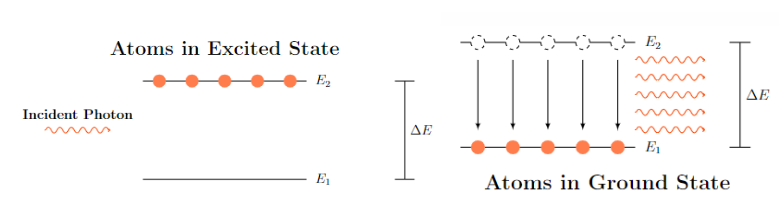
\includegraphics[scale=.78]{./img/07_amplification.png}
    \caption{Stimulated emission from multiple excited atoms in an energy level diagram.}
\end{figure}

The incident photon stimulates the first excited atom, resulting in two in-phase photons traveling in the same direction. These two photons then stimulate two other excited atoms, resulting in four in-phase photons travelling in the same direction. These four photons stimulate four more excited atoms, resulting in eight in-phase photons travelling in the same direction, and so on, creating a chain reaction and a bunch of photons traveling in the same direction resulting in the amplification of light. \vspace{.3cm}

Although this may sound simple, there is a lot going on in reality that we need to take into account. Starting with the fact that the diagrammatic representation of this process in Figure (7) is only from the perspective of energy levels (i.e., energy level diagrams), as we have already discussed, these atoms are actually scattered throughout the system. Therefore, achieving unidirectional, highly collimated, monochromatic, coherent light (i.e., laser light) in reality requires a great deal of work in the construction of a laser.

\subsection{Construction of a Laser}


\begin{figure}[H]
    \centering
    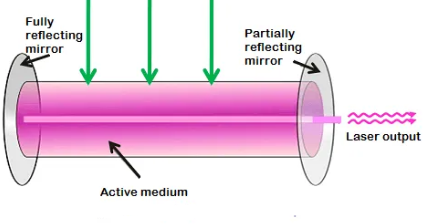
\includegraphics[scale=.9]{./img/09_active_medium.png}
    \caption{Simple diagrammatic representation of Laser}
\end{figure}

This diagram shows a very simplistic model of a LASER based on the very first lasers humans built. In this diagram, the \textbf{Active medium} (or \textbf{Gain medium}) is where the lasing process takes place. \vspace{.2cm}

Anyway, at present, the modern lasers available are very compact and use several methods to improve efficiency but the fundamental principles of lasing process used in the very first lasers are still used.

\subsubsection{Population Inversion}

We learnt that in a system under Thermodynamic equilibrium, there are more atoms in the ground state than in the excited state (according to Boltzmann's law). But to amplify light through stimulated emission, we need more atoms in the excited state to make it more probable for photons to find its way to an excited atom and amplify the radiation. \vspace{.2cm}

\uline{Why do we have to make it more probable for photons to stimulate the atoms?} Because, if not, photons will take a lot of time to find excited atoms and stimulate it resulting in a very low intensity laser beam (which we are not interested in). \vspace{.2cm}

So, we have to make the system (i.e. active medium in the laser) to undergo non equilibrium conditions by supplying energy (represented by green arrows in Figure (8)) to the system from an external source. This process is called as \textbf{Pumping}. \vspace{.2cm}

The supplied energy excites alot of atoms in the ground state to the excited state thus making more atoms to be in excited state than in the ground state resulting in a \textbf{Population Inversion}. This makes it more probable for the photons to find the excited atoms and amplify the radiation more. \vspace{.2cm}

\begin{figure}[H]
    \centering
    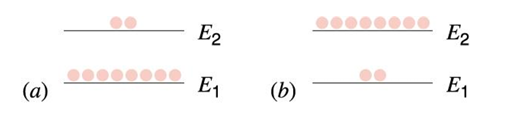
\includegraphics[scale=.8]{./img/10_population_inversion.png}
    \caption{System under equilibrium (a) and System after population inversion (b)}
\end{figure}

\subsubsection{Metastable states}

When an atom excites to an excited state, it becomes very unstable and tends to de-excite spontaneously (almost instantly). The average time for which an atom remains in an excited state is $10^{-8}\,\text{s}$, after which it de-excites spontaneously. This is a problem because the atom gets de-excited spontaneously before even the photon reaches the atom to de-excite it through stimulation and amplify the radiation.
\vspace{.2cm}

There are certain exceptional energy states in certain elements where the average time taken for an atom to remain in those energy states are as high as $10^{-3}s$ which is large enough (compared to $10^{-8}s$) for photons to excite it through stimulation. Theses states are called as \textbf{Metastable states}. \vspace{.2cm} 

This is why active medium in the lasers consists of atoms or ions with such exceptional \textbf{Metastable states} to absorb energy and undergo stimulated emission which increases the output of the laser beam by being excited for long time and making it more probable for a photon to stimulate an excited atom.

\subsubsection{Directionality and Coherence}

One of the most important aspect of laser is that how it's beam is highly collimated and coherent. This is achieved by the way how lasers are constructed. \vspace{.2cm}

When pumping takes place, alot of atoms in the active medium gets excited. Initially, there will not be many photons in the active medium to start the chain of stimulated emission so few excited atoms in the active medium have to undergo spontaneous emission releasing photons. We know, in spontaneous emissions, photons are emitted in various directions. But, we need our laser beam to be highly collimated so we have to filter out photons which are not travelling parallel the axis of the active medium. \vspace{.2cm}

If you observe Figure 8, the active medium is enclosed by two mirrors on either side, with its length exposed. Photons that do not travel parallel to the axis of the active medium undergo several reflections between the mirrors and eventually escape the medium. In contrast, photons traveling parallel to the axis remain perpendicular to the mirrors. Even after multiple reflections, they stay in the same line, allowing only the photons traveling parallel to the axis to remain within the active medium.

\end{document}